\chapter{Raspberry Pi Car}
%https://www.matec-conferences.org/articles/matecconf/pdf/2017/39/matecconf_cscc2017_02025.pdf

%https://www.wseas.org/multimedia/journals/power/2017/a465916-072.pdf


\section{Hardware}
Für die Umsetzung des Projekts wird ein 1:10 ferngesteuertes Modellauto und ein Raspberry PI 3B+ mit Kameramodul verwendet. Auf die genaue Verwendung der genannten Komponnenten wird im Weiteren eingegangen. 

\subsection{Raspberry Pi}
\begin{figure}
\centering
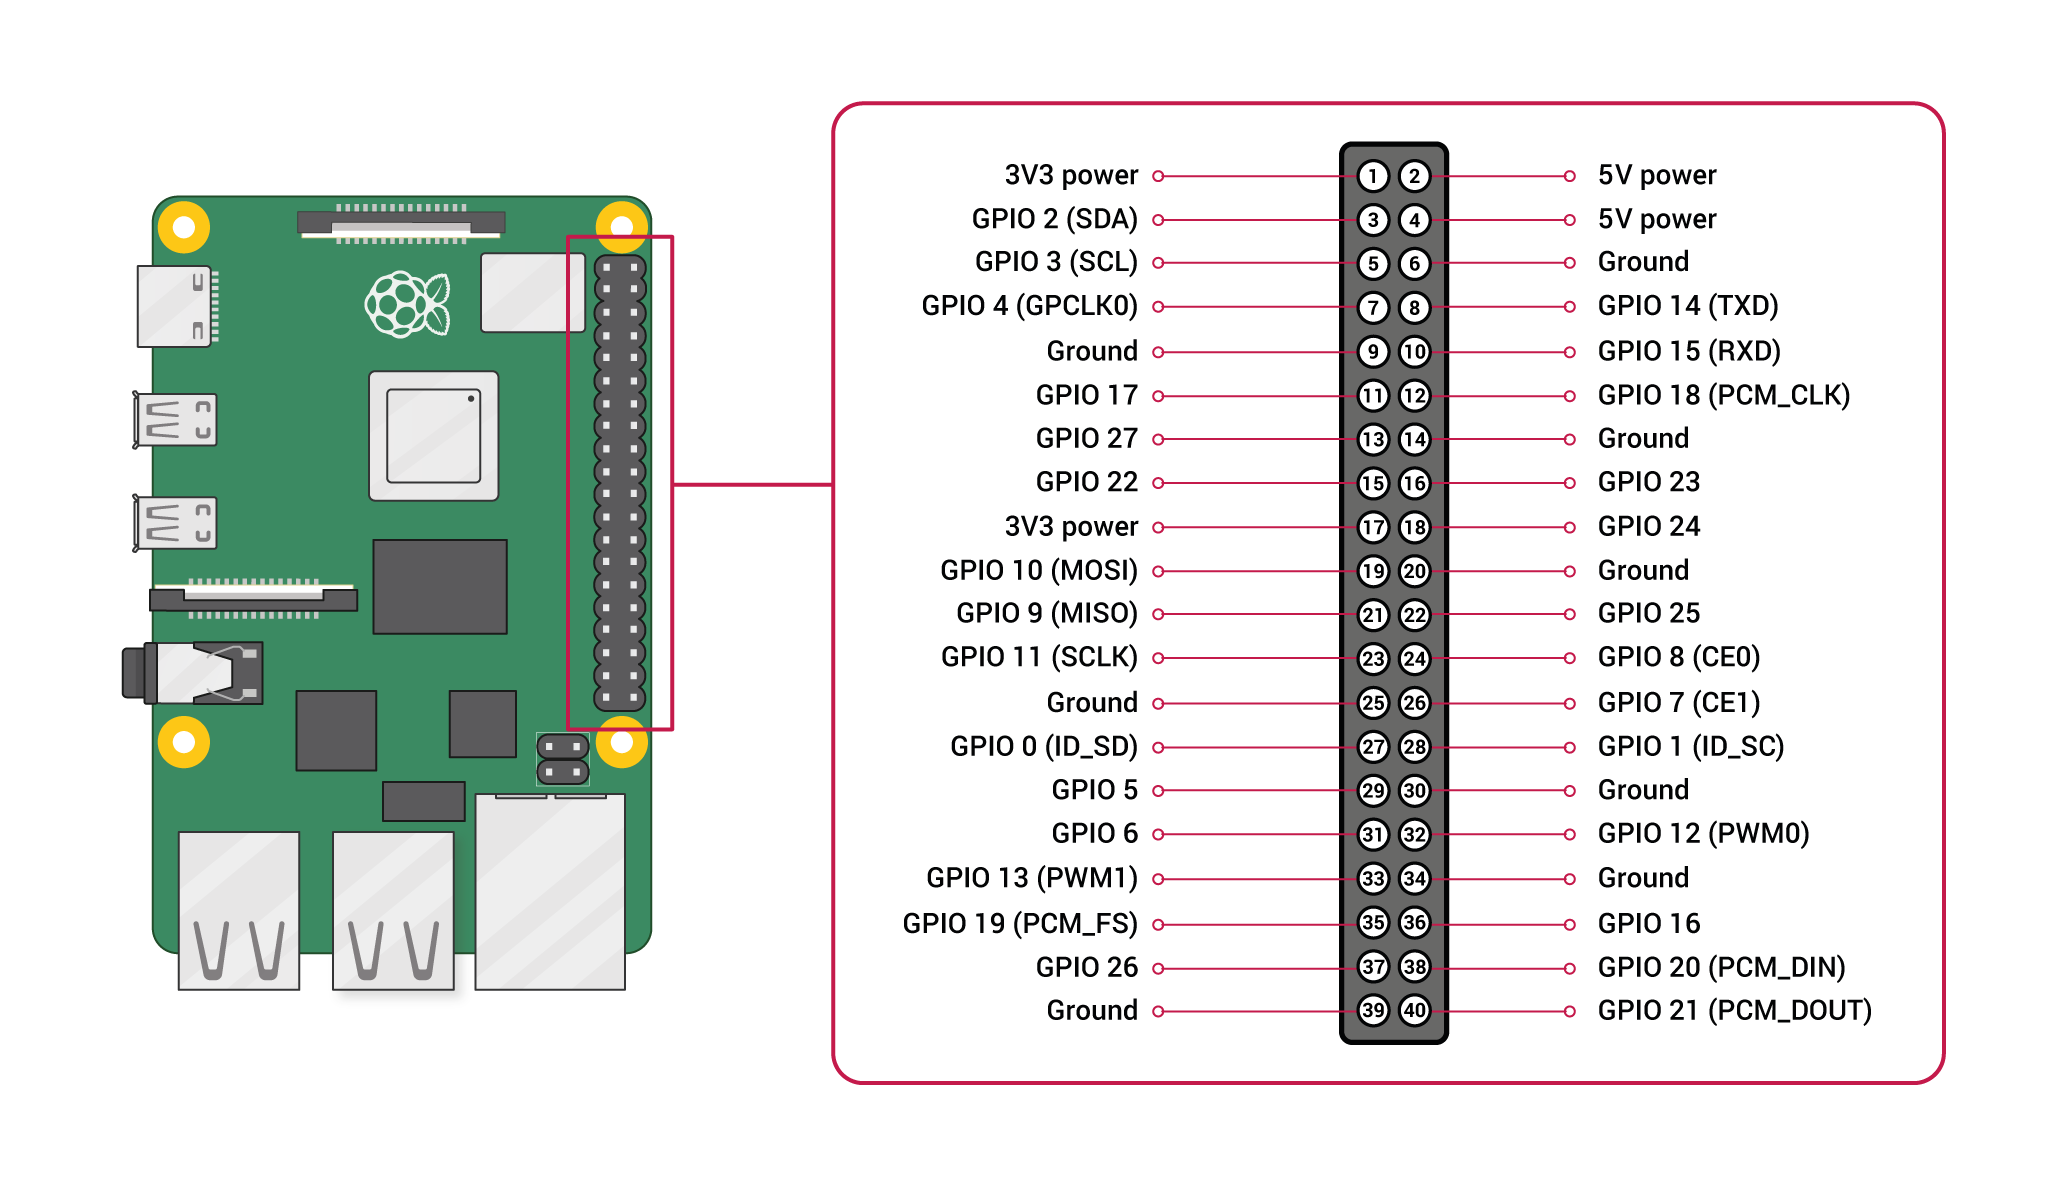
\includegraphics[width=\textwidth]{\imagedir/Raspberry.png}
\caption{Raspberryboard \autocite[VglRaspberrboard]{https://www.raspberrypi.org/documentation/usage/gpio}} 
\end{figure}
Ein \ac{Pi} ist ein Minicomputer mit Betriebssystem in Kreditkartengröße. Er verfügt unter anderem über USB-Anschlüsse, einen HDMI-Port, sowie einen Anschluss für ein Kameramodul. Desweiteren verfügt der \ac{Pi} über \ac{GPIO}-Ports die über Programmiersprachen, wie zum Beispiel Python mit den entsprechenden Bibliotheken, angesteuert werden können. 

Für dieses Projekt wird Raspberry Pi OS als Betriebssystem auf einer 8 Gb microSD und eine 10.000 mAh Powerbank zum Betreiben des \ac{Pi}'s genutzt.

Der \ac{Pi} bildet das Herzstück des \ac{SELMA}. Mit Hilfe des Kameramodul werden Bilder aufgenommen, die durch die Softwarekomponenten Lanedetection und Objectdetection ausgewertet werden, um mit deren Ausgaben das Modellauto zu steuern.

Die Programmierung findet hauptsächlich außerhalb des \ac{Pi}'s auf den Laptop's der Gruppenteilnehmer statt. Um den Code auf den \ac{Pi} zu spielen, wird dort das Github des Projekts gecloned und fortlaufend aktualisiert. Zur Erleichterung bei kleinen Änderungen auf dem \ac{Pi} kommen eine USB Maus, Tastatur und ein externer Monitor zum Einsatz.

\subsection{Modellauto}
Das Modellauto besteht aus den Komponenten: Lenkservo, Funkfernsteuerung, Empfänger, Motor, Fahrtenregler und Akku. Die Steuerung funktioniert im eigentlichen Sinne über die Funkfernsteuerung welche Signale an den Empfänger sendet. Dieser wird über die Verbindung des Fahrtenreglers mit Strom versorgt und versorgt seinerseits den Lenkservo mit Strom. Die Verbindung zu Lenkservo und Fahrtenregler besteht aus jeweils drei Adern. Zwei dienen der Stromversogung, wie bereits beschrieben, die dritte Ader dient der Ansteuerung der beiden Komponenten. Über diese Ader werden \ac{PWM} Signale in einer bestimmten Frequenz übermittelt. \ac{PWM} ist eine digitale Modulationsart, bei der in gegebener Frequenz ein Intervall in bestimmter Dauer übermittelt.

\begin{figure}[H]
\centering

\includegraphics[width=\textwidth]{\imagedir/PWM.png}
\caption{Raspberryboard \autocite[VglRaspberrboard]{https://www.raspberrypi.org/documentation/usage/gpio}} 
\end{figure}

Je nach Intervalldauer gibt beispielsweise der Fahrtenregler Gas beziehungsweise lenkt das Lenkservo.

\subsection{Verkablung}
Um das Modellauto mit dem \ac{Pi} zu steuern, muss die Übermittlung der \ac{PWM} Signale vom \ac{Pi} geschehen. Um dies zu realisieren, wird der \ac{Pi} zwischen den Empfänger und den Lenkservo beziehungsweise dem Fahrtenregler eingelötet. Um die \ac{PWM} Signale vom \ac{Pi} zu übermitteln, muss jeweils für Lenkservo und Fahrtenregler, ein Minuskabel und die dritte Arder, für die Signalübertragung, mit dem \ac{Pi} anstatt dem Empfänger verbunden. Im folgenden ist die Verbindung zwischen allen Komponenten visuell dargestellt:
\begin{figure}[H]
\centering
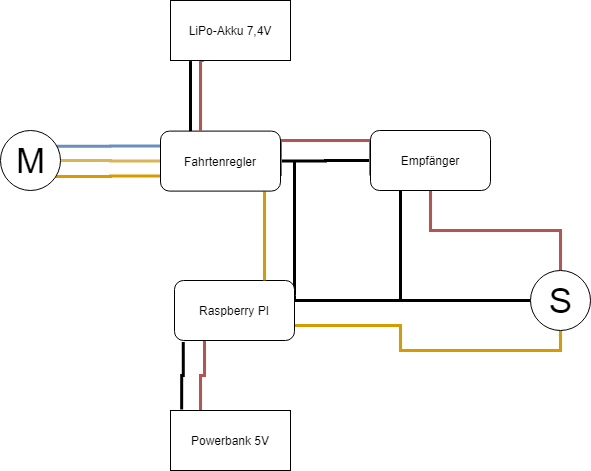
\includegraphics[width=\textwidth]{\imagedir/Schaltplan.jpg}
\caption{Raspberryboard\autocite[Vgl https://www.raspberrypi.org/documentation/usage/gpio]{}} 
\end{figure}

\subsection{Ansteuerung der \ac{GPIO}-Pins mit Python}\label{ss:Ansteuerung}
Für die Umsetzung der Ansteuerung wird die RPi.GPIO Bibliothek und die Pins 33 und 35 für Fahrtenregler und Lenkservo genutzt. Die \ac{PWM} Signale werden in einer 50 Hertz Frequenz übermittelt. Hierbei muss besonderes Augenmerk auf die korrekte Frequenz gelegt werden, da sonst die Elektronik des Lenkservos beziehungsweise des Fahrtenreglers durchbrennen kann. Dies ist bei der Umsetzung des Projektes leider zweimal mit Lenkservos geschehen. Im Folgenden werden die Kernbestandteile der \ac{PWM}-Ansteuerung erklärt. Die volle Ansteuerung ist im Anhang unter \ref{c:steeringcontroll} zu finden.

\begin{lstlisting}[language=Python]
IO.setmode(IO.BOARD)
IO.setup(35,IO.OUT)
steering =IO.PWM(35,50)
steering.start(0)
\end{lstlisting}
Mit den obigen Befehlen wird die Ansteuerung des \ac{PWM}-Pin 35 mit einer 50 Hertz-Frequenz initiiert. Die Aktivintervalldauer (duty cycle) wird dabei auf 0 gesetzt.

\begin{lstlisting}[language=Python]
steering.ChangeDutyCycle(10)
steering.stop()
\end{lstlisting}
Mit der Funktion ChangeDutyCycle kann die Dauer des Aktivenintervalls (duty cycle) verändert werden. In diesem Beispiel wird die Zeit des Aktivenintervalls auf 10\% der Intervalldauer gesetzt. Mit der Funktion stop wird die Ansteuerung des entsprechenden \ac{GPIO}-Pins gestoppt.


\section{Steuerung des Modellautos}

%https://link.springer.com/chapter/10.1007/978-1-4842-5174-4_1
Introduction to machine learning (ML) with the Raspberry Pi (RasPi)

Für die Steuerung des Modellautos wird das run\_car.py Skript genutzt. Dieses nutzt die Kamera um ständig Bilder aufzunehmen und diese zur Steuerung auszuwerten. Dazu werden die bereits erklärten Funktionen aus object- und lane\_detection genutzt. Darüber hinaus wird ein Car-Objekt erzeugt, mit dem das Modellauto angesteuert werden kann. Dies wurde in \ref{ss:Ansteuerung} erläutert.
\newline
Die Auswertung der Kamerabilder werden in einer While-Schleife durchgeführt. Dazu wird zu Beginn der While-Schleife ein Bild mit der Kamera erstellt. Dieses wird dann, falls kein Thread zur Objekterkennung läuft, an einen neune Thread zur Objekterkennung übergeben. Dieser läuft asynchron und blockiert nicht den weiteren Ablauf und die Auswertung zur Steuerung des Autos. Nach dem, falls notwendig, der Objekterkennungsthread gestartet wurde, wird das Bild mit Hilfe der lane_detection Funktion aus dem lanedetect_steer Skript ausgewertet. Die Funktion gibt einen Anweisung zur Steuerung des Modellautos zurück. Diese Anweisung wird genutzt um mit der Steer-Methode das Modellauto zu steuern. Der Objekterkennungsthread liefert einen Boolean zurück. Sollte die Booleanrückgabe True sein, wird das Auto angehalten und erst wieder gestartet, wenn die Rückgabe False ist. 